\documentclass[polish,polish,a4paper]{article}
\usepackage[T1]{fontenc}
\usepackage[utf8]{inputenc}
\usepackage{babel}
\usepackage{pslatex}
\usepackage{graphicx}
\usepackage{tikz}
\usepackage{pgfplots}
\usepackage{anysize}
\usepackage{pgfgantt}
\usepackage{tabularx}
\usepackage{float}
\usepackage{latexsym,amsmath}
\marginsize{2.5cm}{2.5cm}{3cm}{3cm}


\newcommand{\name}[1]{\sffamily\bfseries\scriptsize #1}

\newcommand{\frontpage}[8]{
%% #1 - nazwa kursu
%% #2 - kierunek 
%% #3 - termin 
%% #4 - temat 
%% #5 - problem
%% #6 - data

\vspace{2cm}

\begin{tabular}{|p{0.72\textwidth}|p{0.28\textwidth}|}
\hline
\multicolumn{2}{|c|}{}\\
\multicolumn{2}{|c|}{{\LARGE #1}}\\
\multicolumn{2}{|c|}{}\\
\hline
\name{Kierunek} & \name{Termin}\\
\multicolumn{1}{|c|}{\textit{#2}} & \multicolumn{1}{|c|}{\textit{#3}} \\
\hline
\name{Temat} & \name{Problem}\\
\multicolumn{1}{|c|}{\textit{#4}} & \multicolumn{1}{|c|}{\textit{#5}} \\
\hline
\name{Prowadzący} & \name{data}\\
\multicolumn{1}{|c|}{\textit{mgr inż. Radosław Idzikowski}} & \multicolumn{1}{|c|}{\textit{#6}} \\
\hline
\end{tabular}

}

\usepackage{listings}
\usepackage{xcolor} % for setting colors



% set the default code style
\lstset{ % General setup for the package
	basicstyle=\small,
	numbers=left,
	frame=tb,
	tabsize=2,
	columns=fixed,
	showstringspaces=false,
	showtabs=false,
	keepspaces,
	commentstyle=\color{red},
	keywordstyle=\color{blue}
}

\title{Sprawozdanie SPD}
\begin{document}
% #1 - nazwa kursu #2 - kierunek  #3 - termin #4 - temat #5 - problem #6 - data
\frontpage{Projektowanie Efektywnych Algorytmów}{Informatyka}{Czwartek 19:05}{Metoda przeglądu zupełnego, podzialu i ograniczeń, oraz programowanie dynamiczne.}{TSP}{\today}
\pagestyle{empty}
\newpage

\section{Opis problemu}

Problem komiwojażera (ang. travelling salesman problem, TSP) jest zagadnieniem optymalizacyjnym, polegającym na znalezieniu minimalnego cyklu Hamiltona w pełnym grafie ważonym\cite{TSPWiki:1}. Do rozwiązania problemu tym razem autor posłużył się dwoma algorytmami aproksymacyjnymi o których szerzej w dalszej częsci.
Do implementacji rozwiązania posłużył język C++, gdyż zdaniem autora pozwala on na wygodne opisywanie wysokopoziomowej abstrakcji oraz dostępne kompilatory
potrafią generować efektywny kod. Testy przeprowadzane były na systemie Ubuntu Linux 19.10 64bit z kompilatorem clang 9.0 na procesorze Intel i5-3570K (4x3.8GHz) z 8GB RAM.

\section{Struktury danych - sposób przechowywania informacji}

\subsection{Graf}

Problem komiwojażera można zdefiniować dla różnej ilości wieszchołków, dalej nazywaną wielkością problemu oraz różnych wag poszczególnych dróg łączących te wierzchołki.
Z tego względu wymaganym mechanizmem wczytywania informacji o problemie będzie plik, który zawiera wielkość grafu oraz wagi poszczególnych wierzchołków.
Wagi podawane są w postaci macierzy, w której kolejne elementy w wierszu oddzielane są znakami białymi, a same wiersze oddzielane są znakiem nowej lini.
Tak zapisane dane należy sparsować i zapisać w postaci pozwalającej na jak najprostszy oraz najszybszy sposób odczytu, ponieważ będzie ona intensywnie wykorzystywana przy rozwiązywaniu problemu.
Autor zdecydował się na przechowywanie danych w postaci kwadratowej macierzy sąsiedztwa o rozmiarze równym ilości wierzchołków.
I do jej reprezentacji została wykorzystana pojedyncza tablica typów int64\_t o rozmiarze $N^{2}$, gdzie N to rozmiar problemu.
Poniżej znajduje się definicja klasy MSTMatrix która implementuje przechowywanie macierzy sąsiedztwa.

\lstinputlisting[caption=Struktura danych MSTMatrix,language=C++]
{mst.hpp}

Jeden drobny szczegół pozostaje nie wyjaśniony - typ Edge, który klasa MSTMatrix przyjmuje jako argument przy metodzie dodawania krawędzi do grafu.
Jej implementacja jest prosta i sprowadza się do przetrzymywania informacji numeru wierzchołka źródłowego i docelowego, oraz wagi opisywanego połączenia.
Metoda MSTMatrix::add korzysta z jej pól, aby odpowiednio wypełnić informacje we własnej macierzy sąsiedztwa.
Rozwiązanie problemu będzie zwracane jako typ Path ktory jest lekkim wrapperem na klase std::vector z standardowej biblioteki.
Jego implementacja znajduje sie poniżej.

\lstinputlisting[caption=Struktura danych Path,language=C++]
{path.hpp}

Został jeszcze jeden element który wymaga krótkiego wyjaśnienia. Jest to funkcja kosztu scieżki która zwraca koszt danej scieżki na podstawie argumentu w postaci macierzy sąsiedztwa
oraz sekwencji kolejno odwiedzanych wierzchołków.

\section{Metoda przeszukiwania tabu (ang. Tabu search)}

Przed omówieniem działania algorytmu przeszukiwania tabu wprowadzona musi zostać definicja ruchu (ang. move) oraz
sąsiedztwa danego rozwiązania (ang. local neighborhood).

\subsection{Operacja ruchu (ang. move)}
Operacją ruchu nazywamy taką operację na dwóch wierzchołkach istniejącego, poprawnego rozwiązania, która za pomocą dowolnych,
deterministycznych operacji zmieni szyk (kolejność) wierzchołków w drodze. W tym przypadku autor zdecydował się na implementację
trzech różnych strategii dokonywania opsiywanego ruchu. Są to zamiana wierzchołków (ang. swap), lustrzane odbicie rozpatrując 
kolejność występowania wierzchołków w zakresie wyznaczonym przez wierzchołki bedące argumentem opreacji (ang. reverse) (np.
dla sekwencji ABCDEF i argumentów B oraz E otrzymamy AEDCBF - kolejność wierzchołków w zakresie od B do E została odwrócona),
oraz wstawienie jednego z późniejszego w sekwencji z wierzchołków przed wcześniejszego (ang. insert). Wszystkie strategie są
łatwo konfigurowalne, oraz ich konfiguracja nie wpływa na czas wykonania programu (przekazywane są jako parametr szablonu).
Dla każdej z nich została przeprowadzona osobna analiza skuteczności. Implementacja każdej z nich znajduje na kolejnych listingach.

Każda operacja zamiany zaimplementowana jest jako funktor który przekazywany jest do klasy odpowiedzialnej za rozwiązanie problemu.
Każdy z funktorów potrafi przeprowadzić nie tylko sam ruch, ale również spekulację na temat jego opłacalności. Taka operacja 
przydatna jest przy szukaniu najlepszego sąsiada bez decydowania się od razu na ruch. Przez to, że ruch operuje już na istniejącej
i poprawnej ścieżce (i generuje z niej kolejną poprawną) pozostaje problem wyznaczenia drogi początkowej od której ta metoda może
rozpocząć działanie. Autor zdecydował się na bardzo podobny zabieg i w tym przypadku. Tak jak wcześniej mamy tutaj parametr szablonu
, który determinuje sposób w który początkowa droga zostanie wylosowana. Dostępnymi sposobami generowania początkowej scieżki są:
zwyczajna droga składająca się z kolejnych wierzchołków od pierwszego do ostatniego, rozpoczęcie od wierzchołka zerowego oraz
kolejne, zachłanne dołączanie sąsiada o lokalnie najtańszym koszcie przejscia, oraz droga (pseudo)losowa. Ich implementacja jest
trywialna i autor zdecydował się nie zamieszczać ich implementacji w sprawozdaniu. Ich implementacja jest dostępna w publicznym
repozytorium.

\pagebreak
\lstinputlisting[caption=Zamiana wierzchołków (ang. swap),language=C++]
{swap_op.cc}

\pagebreak
\lstinputlisting[caption=Odbicie (ang. reverse),language=C++]
{invert_op.cc}

\pagebreak
\lstinputlisting[caption=Wstawienie (ang. insert),language=C++]
{insert_op.cc}

\subsection{Sąsiedztwo rozwiązania (ang. neighborhood)}
Sąsiadem rozwiązania nazywamy takie rozwiązanie, które można otrzymać poprzez pojedynczą operacji ruchu z udziałem dowolnych
dwóch różnych wierzchołków.

\subsection{Implementacja przeszukiwania}
Po zdefiniowaniu potrzebnych pojęć, sama implementacja algotytmu jest relatywnie prosta. Po zainicjowaniu odpowiednich struktur
danych i wytworzeniu początkowej scieżki rozpoczyna się głowna pętla algorytmu, której ilość iteracji wpada w obszar kalibracji
implementacji i nie jest jednoznaczna. Autor w tej konkretnej implementacji zdecydował sie na 10'000 interacji. W pętli następuje
przejscie po wszystkich możliwych kombinacjach dwóch wierzchołkach które będą kandydatami do bycia najlepszym sąsiadem.
Koszt hipotetycznego ruchu z użyciem danych dwóch wierzchołków zostaje zapisany jeżeli jest tańszy od aktualnie najtańszego, aby
na koniec można było wykonać najbardziej opłacalny ruch. Uważny odbiorca jest w stanie zauważyć, że podążając tym alorytmem możemy
znaleźć lokalnie najlepszego sąsiada, ale gorszego niz aktualne rozwiązanie przez co ostatecznie zboczyć na gorsze rozwiązanie.
Z tego powody dodatkowo przechowywana jest globalnie najlepsza scieżka jaka była widziana w czasie działania całego algorytmu i to
ona jest (oczywiście) aktualizowana w trakcie działania algorytmu oraz ostatcznie zwracana jako ostateczne rozwiązanie.
Gdy najlepszy kandydat ruchu został znaleziony, oraz sam ruch został wykonany, dodatkowo dwa wierzchołki, które wchodziły w ruch
zostają dodane do tablicy tabu i warunkowo (o tym więcej później) zablokowana na, w przypadku tej konkretnej implementacji 5
iteracji pętli. Ruch który znajduje się na liście tabu może zostać wykonany jeżeli oferuje "bardzo atrakcyjny" ruch. Atrakcyjność
ruchu wyznaczana jest na podstawie jego kosztu (podstawowe kryterium) i dodatkowo obarczone jest kosztem tym większym im większa
wartość w liście tabu widnieje dla danego ruchu (z każdą iteracja koszt tabu ulega dekrementacji do momentu aż ruch nie osiągnie
wartości 0 i zostanie uznany jako usunięty). Sama lista tabu zaimplementowana jest jako macierz, która posiada wartość tabu dla
połączenia każdego wierzchołka z każdym. Taka implementacja pozwala na szybkie odczytanie kosztu danego ruchu w trakcie jego
wykonywania. Pozostaje jedynie kwestia dekrementacja wartości tabu w liście. Z każdym obiegiem pętli algorytm musiałby przejsc
po wszystkich elementach i odpowiednio zmodyfikować ich wartość. Autor jednak zdecydował się nieznacznie zmienić implementacje
listy tabu i zamiast wartości tabu wpisywać tam numer interacji pętli w ktorym dane połączenie bedzię usunięte z listy tabu.
Można o tym myśleć jak o punkcie czasowym w jakim dane ruch zostanie uznany jako usunięty z listy. Dla przykładu:
Jeżeli aktualny numer iteracji głownej pętli równy jest 10 i właśnie dokonaliśmy ruchu to należy wpisac go do listy tabu z wartością
10 + 5 = 15. Gdzie wartość 5 wynika z tej konkretnej implementacji algorytmu. Wówczas funkcja pobierająca koszt tabu dla danego
ruchu polega na odjęciu od znalezionej tam wartości, aktualnej wartości iteracji pętli. Implementacja operacji na liście tabu
została załączona na listingu "Implementacja listy tabu - sztuczka optymalizacujna" (został uszczuplona o nieistotne szczegóły).
Dodatkowo, żeby zapobiec zatrzymania w loklanych minimach został dodany jescze jeden element do głównej pętli algorytmu.
Jest to licznik iteracji bez znalezienia lepszego rezultatu. Jeżeli ten licznik przekroczy, w przypadku tej implementacji wartość
300 iteracji, nowa droga powstaje przez wylosowanie nowej drogi a nie poprzez wykonanie ruchu. Impelementacja głównej pętli znajduje
się na listingu "Przeszukiwanie tabu - główna pętla algorytmu".

\pagebreak
\lstinputlisting[caption=Implementacja listy tabu - sztuczka optymalizacujna,language=C++]
{tabu_list.cc}

\pagebreak
\lstinputlisting[caption=Przeszukiwanie tabu - główna pętla algorytmu,language=C++]
{tabu_loop.cc}

\pagebreak
\section{Eksperymenty obliczeniowe}
Czas wykonywanych operacji był mierzony na systemie opisanym w wprowadzeniu.
Do pomiaru czasu wykorzystano standardową bibliotekę języka C++, biblioteke std::chrono.
Pomiar czasu wykonywany był w nanosekundach. Każdy pomiar wykonywany był 50 razy i ostatecznym wynikiem była średnia czasu z wszystkich prób.
Dodatkowo przed dokonywaniem takiego pomiaru uruchamiano 10 razy przebieg mierzonego kawałka kodu bez mierzenia jego czasu po to aby wytrenować układy przewidywania odwoływań do pamięci,
tj. branch prediction, cache prefetching.
Poniżej znajduje się kod realizujący mierzenie czasu.

\lstinputlisting[caption=kod metody programowania dynamicznego,language=c++]
{timeutils.hpp}

\pagebreak
\begin{center}
\begin{tabularx}{0.5\textwidth} { 
	| >{\centering\arraybackslash}X 
	| >{\centering\arraybackslash}X | }
	\hline
	\multicolumn{2}{|c|}{Metoda przeglądu zupełnego} \\
	\hline
	Wielkość problemu & Czas wykonania (ns) \\
	\hline
	2 & 328 \\
	\hline
	3 & 691 \\
	\hline
	4 & 3026 \\
	\hline
	5 & 17928 \\
	\hline
	6 & 80026 \\
	\hline
	7 & 442466 \\
	\hline
	8 & 3953679 \\
	\hline
	9 & 39880219 \\
	\hline
	10 & 442507917 \\
	\hline
	11 & 5353492295 \\
	\hline
\end{tabularx}

\bigskip

\begin{tabularx}{0.5\textwidth} { 
	| >{\centering\arraybackslash}X 
	| >{\centering\arraybackslash}X | }
	\hline
	\multicolumn{2}{|c|}{Metoda przeszukiwanuia w głąb} \\
	\hline
	Wielkość problemu & Czas wykonania (ns) \\
	\hline
	2 & 225 \\
	\hline
	3 & 699 \\
	\hline
	4 & 1469 \\
	\hline
	5 & 6033 \\
	\hline
	6 & 21570 \\
	\hline
	7 & 84161 \\
	\hline
	8 & 179542 \\
	\hline
	9 & 730287 \\
	\hline
	10 & 2420364 \\
	\hline
	11 & 5190784 \\
	\hline
	12 & 92879242 \\
	\hline
	13 & 546526194 \\
	\hline
	14 & 103633643 \\
	\hline
\end{tabularx}

\bigskip

\begin{tabularx}{0.5\textwidth} { 
	| >{\centering\arraybackslash}X 
	| >{\centering\arraybackslash}X | }
	\hline
	\multicolumn{2}{|c|}{Metoda dynamiczna Helda-Karpa} \\
	\hline
	Wielkość problemu & Czas wykonania (ns) \\
	\hline
	2 & 205 \\
	\hline
	3 & 854 \\
	\hline
	4 & 2780 \\
	\hline
	5 & 3429 \\
	\hline
	6 & 8669 \\
	\hline
	7 & 22836 \\
	\hline
	8 & 51377 \\
	\hline
	9 & 117697 \\
	\hline
	10 & 288131 \\
	\hline
	11 & 651784 \\
	\hline
	12 & 1481028 \\
	\hline
	13 & 3447888 \\
	\hline
	14 & 7751161 \\
	\hline
	15 & 17600188 \\
	\hline
	16 & 41210060 \\
	\hline
	17 & 94666222 \\
	\hline
	18 & 230991845 \\
	\hline
\end{tabularx}
\end{center}

\newpage

\begin{figure}[H]
\begin{center}
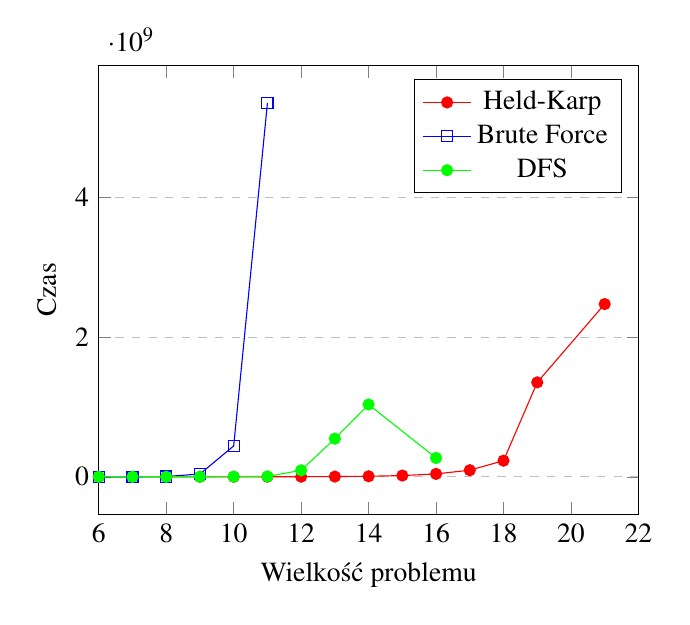
\begin{tikzpicture}
	\begin{axis}[
		xlabel=Wielkość problemu,
		ylabel=Czas,
		ymajorgrids=true,grid style=dashed,
		legend pos=north east,
		xmin=6,
		xmax=22
	]
	\addplot[color=red,mark=*]
	coordinates {
		(2,205)
		(3,854)
		(4,2780)
		(5,3429)
		(6,8669)
		(7,22836)
		(8,51377)
		(9,117697)
		(10,288131)
		(11,651784)
		(12,1481028)
		(13,3447888)
		(14,7751161)
		(15,17600188)
		(16,41210060)
		(17,94666222)
		(18,230991845)
		(19,1353198041)
		(21,2475404238)
	};

	\addplot[color=blue,mark=square]
	coordinates {
		(2,328)
		(3,691)
		(4,3026)
		(5,17928)
		(6,80026)
		(7,442466)
		(8,3953679)
		(9,39880219)
		(10,442507917)
		(11,5353492295)
	};

	\addplot[color=green,mark=*]
	coordinates {
		(2,225)
		(3,699)
		(4,1469)
		(5,6033)
		(6,21570)
		(7,84161)
		(8,179542)
		(9,730287)
		(10,2420364)
		(11,5190784)
		(12,92879242)
		(13,546526194)
		(14,1036336434)
		(16, 270100653)
	};

\legend{Held-Karp, Brute Force, DFS}

\end{axis}
\end{tikzpicture}
\caption{Czas wykonywania się algorytmów w zależności od wielkości problemu}
\end{center}

\begin{center}
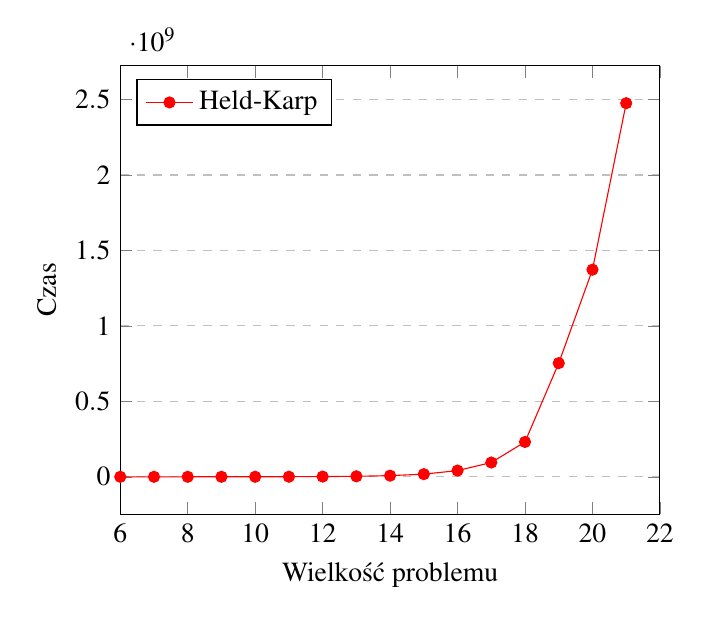
\begin{tikzpicture}
	\begin{axis}[
		xlabel=Wielkość problemu,
		ylabel=Czas,
		ymajorgrids=true,grid style=dashed,
		legend pos=north west,
		xmin=6,
		xmax=22
	]
	\addplot[color=red,mark=*]
	coordinates {
		(2,205)
		(3,854)
		(4,2780)
		(5,3429)
		(6,8669)
		(7,22836)
		(8,51377)
		(9,117697)
		(10,288131)
		(11,651784)
		(12,1481028)
		(13,3447888)
		(14,7751161)
		(15,17600188)
		(16,41210060)
		(17,94666222)
		(18,230991845)
		(19,753198041)
		(20,1372398544)
		(21,2475404238)
	};

\legend{Held-Karp}

\end{axis}
\end{tikzpicture}
\caption{Czas wykonywania się algorytmów w zależności od wielkości problemu}
\end{center}
\end{figure}

\newpage

\section{Wnioski}
\hspace{\parindent}
\par
Algorytm przeglądu zupełnego okazał się być (jak oczekiwano) najmniej efektywnym sposobem rozwiązania problemu. Biorąc pod uwage implementacje generowania permutacji nie jest też
metoda najprostszą do zaimplementowania z tych prezentowanych. Algorytm polega na porównaniu każdej możliwej scieżki wiec jego złożoność to n!, gdyż jest to równoważne z wygenerowaniem
każdej możliwej permutacji zbioru wierzchołków. Metoda jest zwyczajnie nie praktyczna. \\

\par
Algorytm przeglądania drzewa w głąb okazał się być najprostszy do zaimplementowania. Dla każdego nie odwiedzonego jeszcze sąsiada wywołujemy rekurencyjnie procedure.
Dzięki wprowadzeniu dodatkowego sprawdzania aktualnego kosztu drogi możemy wcześniej stwierdzić już na danym etapie, że dane rozwiązanie nie może dać lepszego rezultatu niż najlepszy
dotychas znany, wówczas możemy "odciąć" to rozwiązanie i przejść do sąsiedniego rozgałęzienia. Ta metoda jednak nie daje dużo lepszych rezultatów czasowych. Jest co prawda nieco szybsza,
a tempo wzrostu w praktyce okazuje się dużo bardziej "gładkie", ale nadal nie daje zadowalających rezultatów. Dodatkowo dla różnych danych dostajemy kompletnie różne złożoności, które
wydają się nie być opisywalne żadną uniwersalną złożonością. Wynika to z tego, że sytuacje w których faktycznie "odcinamy" nie opłacalne rozgałęzienia mogą pojawiać się bardzo późno
w trakcie przeszukiwania co prowadzi do tego, że i tak algorytm bedzie musiał przejść przez większość drzewa. \\

\par
Algorytm programowania dynamicznego Helda-Karpa cechuje sie złożonością czasową O($2^nn^2$).
Jego wadą jest jednak duża złożoność pamięciowa ze względu na alokacje dużej tablicy do zapisywania wyników dla podzbiorów wierzchołków, która wynosi O($2^nn$).
Właśnie przez swoją złożoność pamięciową oraz (nadal) długi czas wykonania algorytm nie przydaje sie w praktycznych rozwiązaniach.

\bibliographystyle{abbrv}
\bibliography{ref}
\end{document}

